\section{Scenario editor}
When the editor, which can be found in figure ~\ref{fig:editor}, is opened, two main parts can be seen:
\begin{enumerate}
\item The Configuration panel, which is used to create, open and save configuration files.
\item The Entity panel, where a list of bots and a list of e-partners are being displayed. Here, bots and e-partners can be created, modified, renamed and deleted.
\end{enumerate}

\begin{figure}[h]
\begin{center}
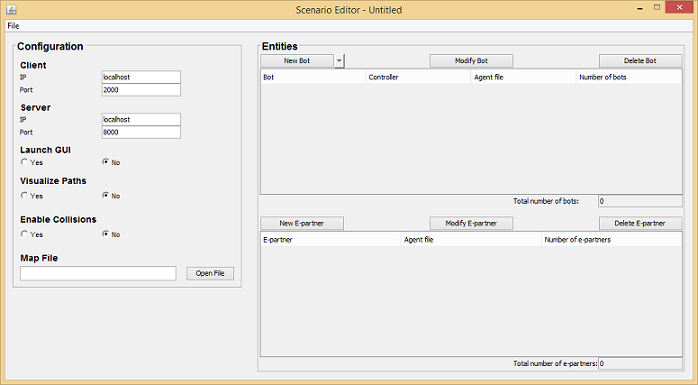
\includegraphics{NewFeatures/editor.png}
\caption{Scenario Editor}
\label{fig:editor}
\end{center}
\end{figure}

\subsection{General use}
At the top of the editor a $File$ menu can be seen. If that is clicked, the options to create a new configuration, open a configuration, save the current configuration, export the current configuration and to exit the editor will be visible.

On the left side of the editor, a scenario can be configured. The Client IP, the Client Port, the Server IP and the Server Port should already contain the default values. These can be changed if needed. It is also possible to indicate whether or not a GUI needs to be opened, if the paths the bots take need to be visualised and if collisions need to be enabled. Map files can also be imported by selecting the $Open$ $file$ button at the right section.

On the right side of the editor bots and e-partners can be created, modified, renamed and deleted. There also are a list of bots and a list of e-partners that are currently created, and below each list there is an indication of how many bots or e-partners are created in total.

Linked to the Scenario Editor are the Bot Store and the E-partner Store, which will also be discussed in this document.

\subsection{Configuration Panel}
A picture of the configuration panel can be found in figure ~\ref{fig:config}.\\\\
\begin{figure}[h]
\begin{center}
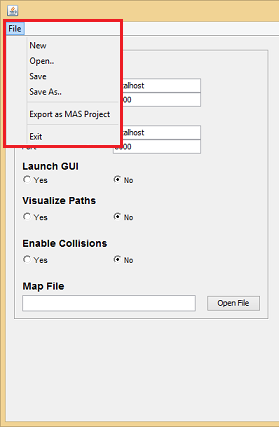
\includegraphics{NewFeatures/config.png}
\end{center}
\caption{Configuration Panel}
\label{fig:config}
\end{figure}
\textbf{New configuration file}
To create a new configuration file, select $File$ $\to$ $New$ in the menu bar. A new configuration with the default values will be created. Creating a new configuration will reset all previous changes made to the configuration, so make sure the current configuration is saved.
\\\\
\textbf{Open configuration file}
To open an existing configuration file, select $File$ $\to$ $Open$ in the menu bar. A window will pop up where the folder can be selected in which the configuration file is saved. Once the right folder is selected, select the file and click the $Open$ button.
\\\\
\textbf{Save configuration file}
To save the current configuration file, select $File$ $\to$ $Save$ in the menu bar. If the current configuration hasn't been saved before, a window will pop up where the folder can be selected to save the configuration file to. Enter a name for the file and click the $Save$ button.
\\\\
\textbf{Save configuration file as}
To save the current configuration in a new file, select $File$ $\to$ $Save$ $As$ in the menu bar. A window will pop up where the folder can be selected to save the configuration file to. Enter a name for the file and click the $Save$ button.
\\\\
\textbf{Export configuration to mas2g}
To export the current configuration to mas2g, the configuration has be first. Once that is done, select $File$ $\to$ $Export$ $as$ $MAS$ $project$ in the menu bar. A window will pop up where the folder to which the configuration will be exported can be selected. Enter the file name and click the $Export$ $MAS$ $project$ button.
\\\\
\textbf{Exit the Scenario Editor}
If the Scenario Editor needs to be closed, select $File$ $\to$ $Exit$ in the menu bar. Closing the Scenario Editor will not save any changes that have been made, so make sure the current configuration is saved first.

\subsection{Entity Panel}
The entity panel exists of 2 parts; the top part shows the bot options and the bottom part shows the e-partner options. A picture of the entity panel can be found in figure ~\ref{fig:bot}.\\\\
\begin{figure}[h]
\begin{center}
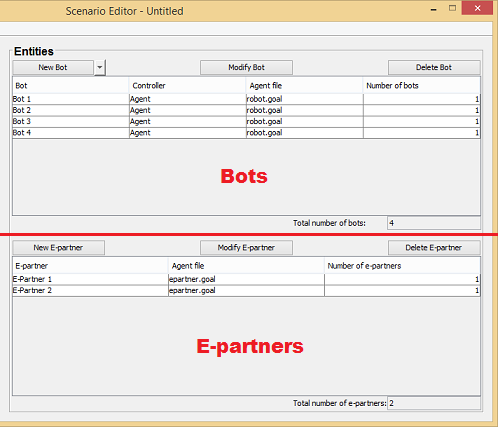
\includegraphics{NewFeatures/bot.png}
\end{center}
\caption{Entity Panel}
\label{fig:bot}
\end{figure}
\textbf{Create new bot}
To create a new bot, click the $New$ $Bot$ button. A new bot will appear in the bot list.\\
If a standard bot needs to be created (which already has default values), click on the arrow next to the $New$ $Bot$ button. A menu will drop down where one of the standard bots can be selected. If one of the standard bots is clicked, the bot will appear in the bot list.
\\\\
\textbf{Modify bot}
To modify a bot, select the bot that needs to be modified in the bot list and click the $Modify$ $Bot$ button. The Bot Store will open in a new window where the properties of the bot can be modified.
\\\\
\textbf{Rename bot}
To rename a bot, either the $Modify$ $Bot$ button can be used to rename in the Bot Store, or the bot can be renamed in the Scenario Editor. To rename in the Scenario Editor, select the bot that needs to be renamed in the list with bots. Double click its name and enter a new name.
\\\\
\textbf{Change controller type}
To change how a bot is controlled, either the $Modify$ $Bot$ button can be used to change it in the Bot Store, or it can be changed in the Scenario Editor. To change the controller type in the Scenario Editor, select the bot that needs to be changed and click on its controller type. The controller type can now be selected.
\\\\
\textbf{Change the amount of entities of a bot}
To change how many entities of a type of bot are created, either use the $Modify$ $Bot$ button can be used to change it in the Bot Store, or it can be changed in the Scenario Editor. To change the entity amount in the Scenario Editor, select the bot that needs its amount changed. Now double click the amount given, and enter a new number.
\\\\
\textbf{Delete bot}
To delete a bot, select the bot that needs to be deleted in the list with bots and click the $Delete$ $Bot$ button.
\\\\
\textbf{Create new e-partner}
To create a new e-partner, click the $New$ $E$-$partner$ button. A new e-partner will appear in the e-partner list.
\\\\
\textbf{Modify e-partner}
To modify an e-partner, select the e-partner that needs to be modified in the e-partner list and click the $Modify$ $E$-$partner$ button. The E-partner Store will open in a new window where the properties of the e-partner can be modified.
\\\\
\textbf{Rename e-partner}
To rename an e-partner, either the $Modify$ $E-partner$ button can be used to rename in the E-partner Store, or it can be renamed in the Scenario Editor. To rename in the Scenario Editor, select the e-partner that needs to be renamed in the list with e-partners. Double click its name and enter a new name.
\\\\
\textbf{Change the amount of entities of an e-partner}
To change how many entities of a type of e-partner are created, either use the $Modify$ $E-partner$ button can be used to change it in the E-partner Store, or it can be changed in the Scenario Editor. To change the entity amount in the Scenario Editor, select the e-partner that needs its amount changed. Now double click the amount given, and enter a new number.
\\\\
\textbf{Delete e-partner}
To delete an e-partner, select the e-partner that needs to be deleted in the e-partner list and click the $Delete$ $E$-$partner$ button.

\subsection{Bot Store}
A picture of the Bot Store can be found in figure ~\ref{fig:bs}.\\\\
\begin{figure}[h]
\begin{center}
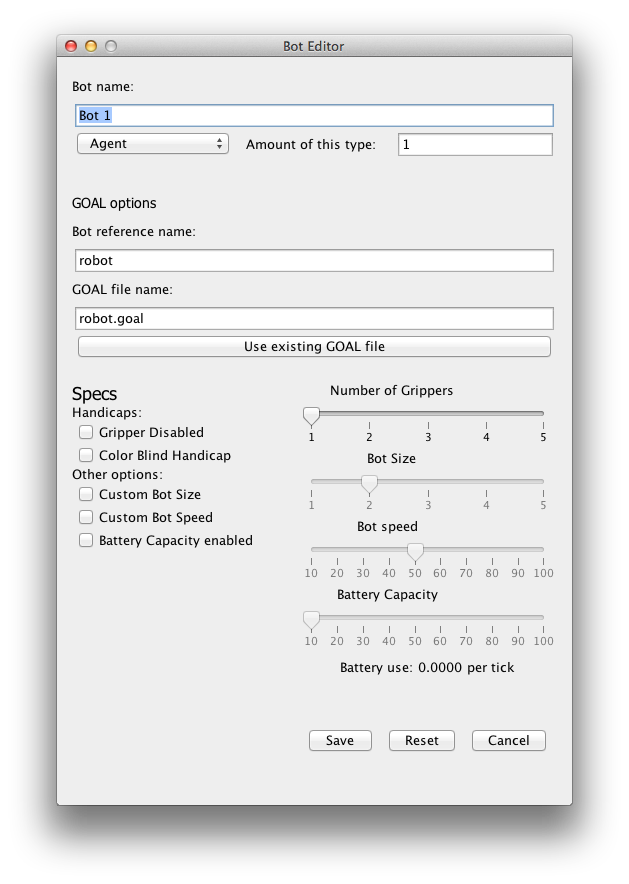
\includegraphics{NewFeatures/bs.png}
\end{center}
\caption{Bot Store}
\label{fig:bs}
\end{figure}
\textbf{Rename bot}
To rename a bot, click on the field that contains its current name. Now the current name is able to be edited or a new name can be entered.
\\\\
\textbf{Change controller type}
To change how a bot is controlled, click its current controller type. Now the controller type can be selected.
\\\\
\textbf{Change the amount of entities}
To change how many entities of the bot need to be created, the field that contains the current number of entities should be clicked. Now the amount is able to be edited.
\\\\
\textbf{GOAL options}
The GOAL options for the bot can be added under the $GOAL$ $options$ section. Here it can be indicated what its reference name in GOAL should be, and a GOAL agent file can be selected which will control the bot. To select the GOAL agent file, click on the $Use$ $existing$ $GOAL$ $file$ button. A window will pop up where the folder in which the GOAL file is saved to can be selected. Once the right folder is selected, select the file and click the $Open$ button.
\\\\
\textbf{Bot properties}
The available bot properties can be found under the $Properties$ section. To change what properties the bot needs to have, select or deselect the checkbox next to the property description. Once a property has been enabled, use the sliders to change the value of that property.
\\\\
\textbf{Save modifications}
If the changes that have been made to the bot need to be changed, click on the $Save$ button. The Bot Store window will close, and the changes will have been saved.
\\\\
\textbf{Reset modifications}
If the changes that have been made to the bot need to be reset, click on the $Reset$ button. The changes will have been reverted to the last saved configuration.
\\\\
\textbf{Cancel modifications}
If modifying the bot needs to be canceled without saving any changes, click on the $Cancel$ button. The Bot Store window will close.

\subsection{E-partner Store}
A picture of the E-partner Store can be found in figure ~\ref{fig:es}.\\\\
\begin{figure}[h]
\begin{center}
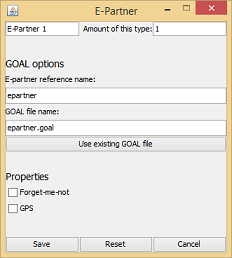
\includegraphics{NewFeatures/es.png}
\end{center}
\caption{E-partner Store}
\label{fig:es}
\end{figure}
\textbf{Rename e-partner}
To rename an e-partner, click on the field that contains its current name. Now the current name is able to be edited or a new name can be entered.
\\\\
\textbf{Change the amount of entities}
To change how many entities of the e-partner will be created, the field that contains the current number of entities should be clicked. Now the amount is able to be edited.
\\\\
\textbf{GOAL options}
The GOAL options for the e-partner can be added under the $GOAL$ $options$ section. Here it can be indicated what its reference name in GOAL should be, and a GOAL agent file can be selected which will control the bot. To select the GOAL agent file, click on the $Use$ $existing$ $GOAL$ $file$ button. A window will pop up where the folder in which the GOAL file is saved to can be selected. Once the right folder is selected, select the file and click the $Open$ button.
\\\\
\textbf{E-partner properties}
The available e-partner properties can be found under the $Properties$ section. To change what properties the e-partner needs to have, select or deselect the checkbox next to the property description.
\\\\
\textbf{Save modifications}
If the changes that have been made to the e-partner need to be changed, click on the $Save$ button. The E-partner Store window will close, and the changes will have been saved.
\\\\
\textbf{Reset modifications}
If the changes that have been made to the e-partner need to be reset, click on the $Reset$ button. The changes will have been reverted to the last saved configuration.
\\\\
\textbf{Cancel modifications}
If modifying the e-partner needs to be canceled without saving any changes, click on the $Cancel$ button. The E-partner Store window will close.
